\subsection{Four-valued robust spacetime compliance}
For uncertain evidence from several sources, membership of one selected point in the authorized region does not suffice to certify the event. We instead impose a set-level requirement: compliance is accepted only if every threshold-supported possible state belongs to the policy and at least one such state exists. Unlike an intersection of all source intervals, this rule allows anomalous intervals to be excluded from the support of an individual state.

For $1\leq k=n-f-r\leq n$, the robust feasible set is
\begin{equation}\label{eq:feasible}
\mathcal F_k=\left\{z\in\Omega:\sum_{i=1}^n\mathbf 1[z\in U_i]\geq k\right\}.
\end{equation}
Here $\mathbf 1[\cdot]$ is the indicator function. Define reachability inside and outside the policy by
\[
I=\mathbf 1[\mathcal F_k\cap P\ne\varnothing],\qquad
O=\mathbf 1[\mathcal F_k\cap(\Omega\setminus P)\ne\varnothing].
\]
The pair $(I,O)$ defines the four mutually exclusive outcomes in Table~\ref{tab:decisions}. Only a Valid classification can authorize acceptance following successful proof verification.

\begin{table}[htbp]\centering\small
\caption{Four-valued robust spacetime compliance.}\label{tab:decisions}
\begin{tabularx}{\linewidth}{@{}ccclX@{}}\toprule
$I$ & $O$ & $\delta$ & Outcome & Feasible-set condition\\\midrule
1&0&0&Valid&$\mathcal F_k\ne\varnothing$ and $\mathcal F_k\subseteq P$\\
0&1&1&Invalid&$\mathcal F_k\ne\varnothing$ and $\mathcal F_k\cap P=\varnothing$\\
1&1&2&Ambiguous&Supported states occur inside and outside $P$\\
0&0&3&Inconsistent&$\mathcal F_k=\varnothing$\\\bottomrule
\end{tabularx}
\end{table}

Inconsistent evidence is a semantic decision computed from a complete set of authenticated signatures. It is not a label for missing signatures, an invalid proof, or an expired nonce. Explicit nonemptiness matters because $\varnothing\subseteq P$ is mathematically true, although an empty feasible set supports no actual event. Conversely, a nonempty feasible set need not contain the physical true state without further assumptions; Section~4 supplies the requisite conditional-soundness argument.

Figure~\ref{fig:counterexample} illustrates how the full-source intersection can disagree with threshold support. Consider $\Omega=[-4,8]\cap\mathbb Z$, $P=[0,8]\cap\mathbb Z$, $n=3$, $f=1$, $r=0$, and $k=2$. Both honest intervals contain the true but noncompliant state $z^\star=-1$. A Byzantine interval excludes this point while leaving the intersection of all three intervals equal to $[2,4]\cap\mathbb Z$. Accepting on that intersection could therefore be incorrect. The threshold-supported set is instead $[-2,4]\cap\mathbb Z$ and spans the policy boundary, correctly producing an Ambiguous decision. This is a constructed illustration of the semantics, not an experimental observation.
\begin{figure}[htbp]\centering
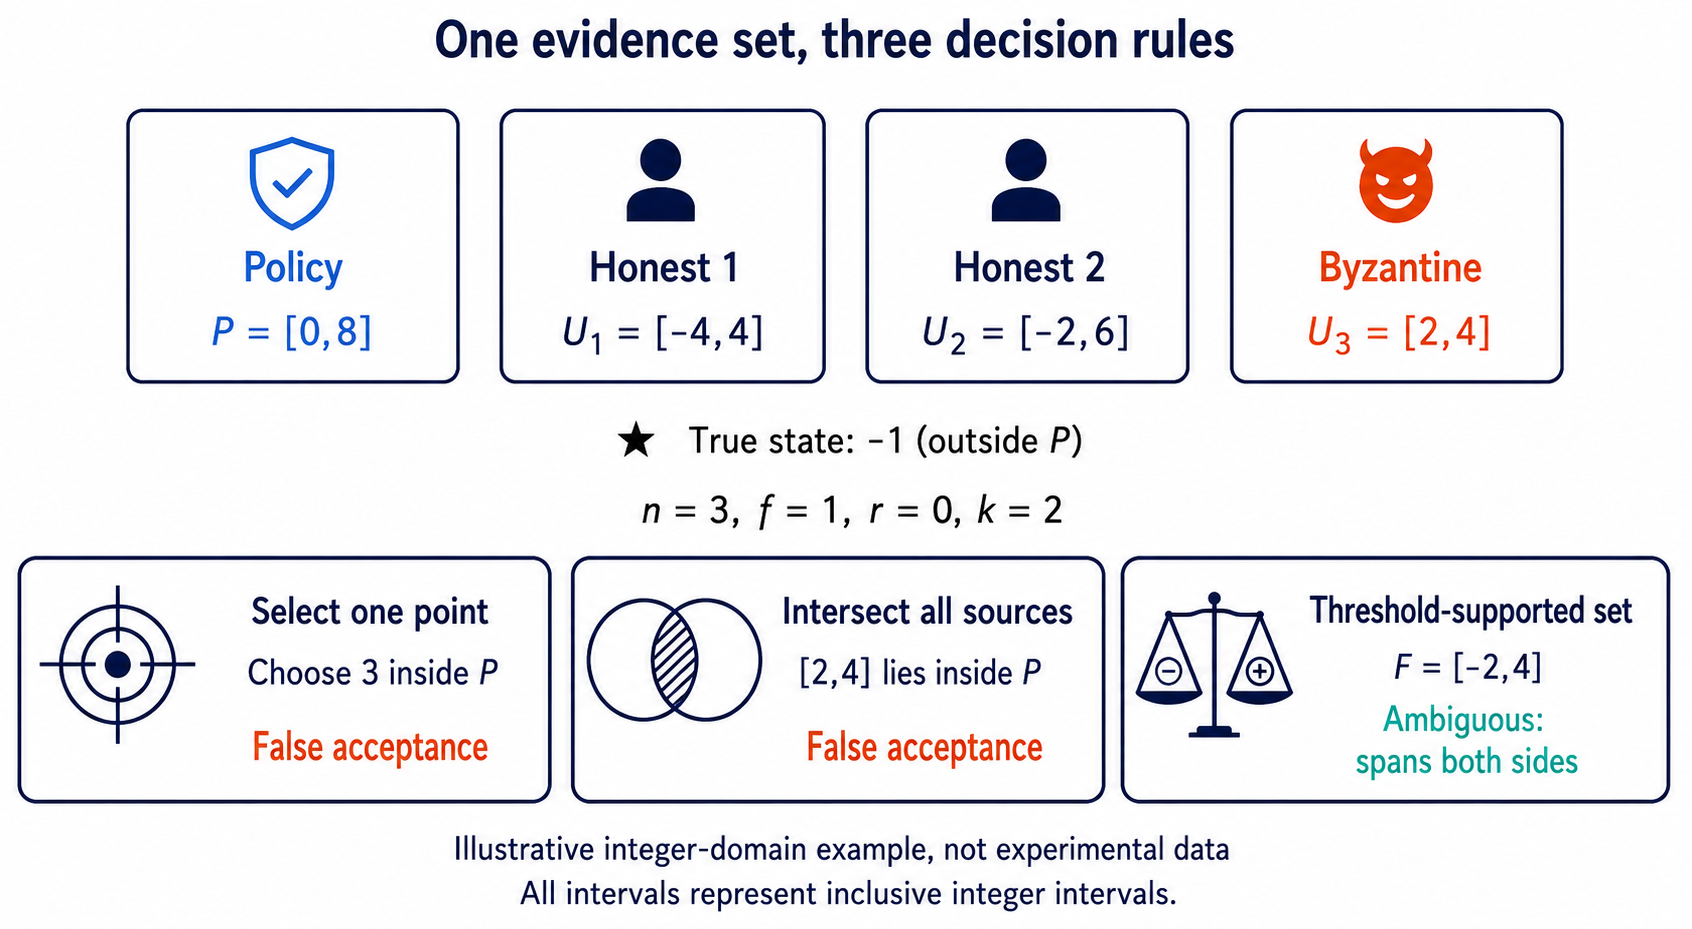
\includegraphics[width=\linewidth]{decision_counterexample.png}
\caption{Three rules applied to the same signed evidence, with inclusive integer intervals and $(n,f,r,k)=(3,1,0,2)$. A selected point or full-source intersection can falsely accept the known noncompliant true state, whereas threshold support yields an ambiguous decision. The example is constructed rather than measured.}\label{fig:counterexample}
\end{figure}
